\documentclass[8pt]{beamer}
\usetheme{Pittsburgh}

\usepackage[backend=biber,style=numeric,autocite=plain,sorting=none]{biblatex}

\usepackage[utf8]{inputenc}

\usepackage{graphicx}
\usepackage{subfigure}
\usepackage{adjustbox}

\usepackage{hyperref}

\usepackage{ragged2e} %\justifying

\PassOptionsToPackage{svgnames,x11names,dvipsnames}{xcolor}
\usepackage[most]{tcolorbox}

\definecolor{softorange}{RGB}{255, 210, 82}
\definecolor{softred}{RGB}{255, 190, 160}
\definecolor{softgreen}{RGB}{125, 240, 210}

\newtcbox{\orangebox}[1][]{enhanced,
 box align=base,
 nobeforeafter,
 colback=softorange,
 colframe=softorange,
 size=small,
 left=0pt,
 right=0pt,
 boxsep=1pt,
 #1}

\newtcbox{\redbox}[1][]{enhanced,
 box align=base,
 nobeforeafter,
 colback=softred,
 colframe=softred,
 size=small,
 left=0pt,
 right=0pt,
 boxsep=1pt,
 #1}

\newtcbox{\greenbox}[1][]{enhanced,
 box align=base,
 nobeforeafter,
 colback=softgreen,
 colframe=softgreen,
 size=small,
 left=0pt,
 right=0pt,
 boxsep=1pt,
 #1}

\setbeamertemplate{bibliography item}{\insertbiblabel}

\setbeamertemplate{footline}[page number]{}

\setbeamertemplate{navigation symbols}{}

\setbeamertemplate{caption}{\raggedright\insertcaption\par}

\AtBeginBibliography{\scriptsize}

\newcommand{\fc}[2]{
	\scriptsize 
	\cite{#1}~\fullcite{#1} \hspace{0.5em}\orangebox{\href{http://home.kerdels.de/#2.pdf}{{\bf PDF}}}~\redbox{\href{http://home.kerdels.de/#2.bib}{{\bf bibtex}}}
}

\newcommand{\vid}[1]{
    \scriptsize
	\greenbox{\href{http://home.kerdels.de/#1}{{\bf video}}}
}

\newcommand{\sof}[2]{{\footnotesize (#1/#2)}}

\newcommand{\twocol}[4]{
\begin{columns}[t]
\begin{column}{#1\textwidth}
#2
\end{column}
\begin{column}{#3\textwidth}
#4
\end{column}
\end{columns}	
}

%%%%%%%%%%%%%%%%%%%%%%%%%%%%%%%%%%%%%%%%%%%%%%%%%%%%%%%%%%%%%%%%%%%%%%%%%%%%%%%%
%%%%%%%%%%%%%%%%%%%%%%%%%%%%%%%%%%%%%%%%%%%%%%%%%%%%%%%%%%%%%%%%%%%%%%%%%%%%%%%%




\begin{frame}{Title \sof{1}{2}}

%\vspace{1em}
\justifying

Foo

\vspace{2em}

% \twocol{0.5}{
% \justifying
% Our technical report~\cite{Dahm2004} provides an in-depth look into the core
% challenges of teaching robots to play soccer, the solutions developed by our
% team, and the involved support infrastructure. 

% \vspace{1em}
% As part of the GermanTeam -- a collaboration between the universities of Berlin,
% Bremen, Darmstadt, and Dortmund -- we won the world championship in the SPL 
% as well as the SPL Open Challenge.

% }{0.41}{
% \vspace{-1.75em}
% \begin{figure}
% 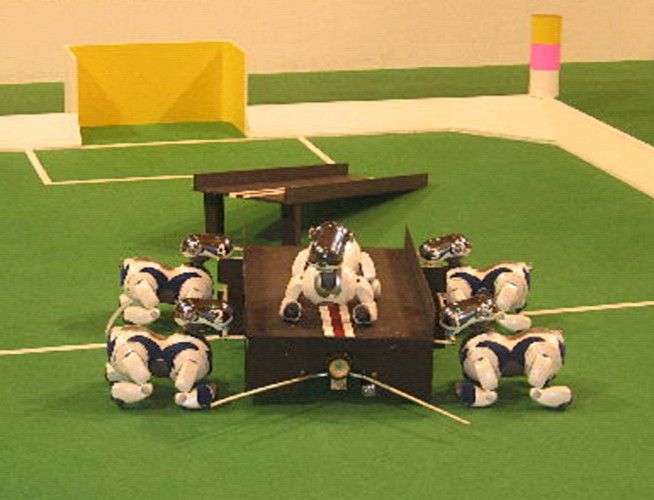
\includegraphics[width=\linewidth]{robocup/robocup.jpg}

% \vspace{-1em}
% \caption{\scriptsize Scene from the SPL Open Challenge~\cite{Dahm2004}.}
% \end{figure}
% }

\vspace{1em}

\begin{center}
\rule{2cm}{0.4pt}\\[0.5em]
\end{center}

\fc{kerdels2013b}{publications/2013-01/2013-01}\nombestpaper\\[1em]
\fc{kerdels2015b}{publications/2015-01/2015-01}\\[1em]
\fc{Kerdels2016}{publications/2016-01/2016-01}\\[1em]
\fc{Kerdels2016a}{publications/2016-03/2016-03}\bestpaper\\[1em]
\fc{Kerdels2016c}{publications/2016-04/2016-04}\nombestpaper\\[1em]
\fc{kerdels2017}{publications/2017-01/2017-01}\\[1em]
\fc{Kerdels2018b}{publications/2018-02/2018-02}\\[1em]
\fcn{Kerdels2018c}{publications/2018-03/2018-03}\\[1em]
\fc{Kerdels2019}{publications/2019-02/2019-02}\\[1em]
\fc{Kerdels2019a}{publications/2019-01/2019-01}

\end{frame}



% The dissertation was featured on the title page of ``Informatik 
% Spektrum''~\cite{Kerdels2018c}, the main organ of the German Informatics 
% Society~(GI).




\begin{frame}{Title \sof{1}{2}}

%\vspace{1em}
\justifying

Foo

\vspace{2em}

% \twocol{0.5}{
% \justifying
% Our technical report~\cite{Dahm2004} provides an in-depth look into the core
% challenges of teaching robots to play soccer, the solutions developed by our
% team, and the involved support infrastructure. 

% \vspace{1em}
% As part of the GermanTeam -- a collaboration between the universities of Berlin,
% Bremen, Darmstadt, and Dortmund -- we won the world championship in the SPL 
% as well as the SPL Open Challenge.

% }{0.41}{
% \vspace{-1.75em}
% \begin{figure}
% 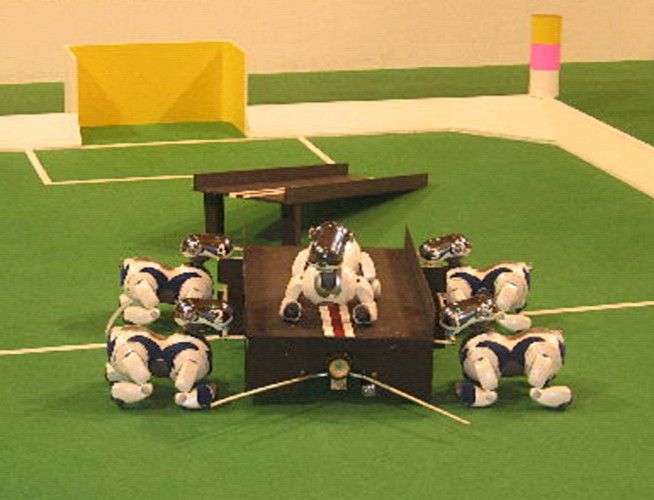
\includegraphics[width=\linewidth]{robocup/robocup.jpg}

% \vspace{-1em}
% \caption{\scriptsize Scene from the SPL Open Challenge~\cite{Dahm2004}.}
% \end{figure}
% }

\vspace{1em}

\begin{center}
\rule{2cm}{0.4pt}\\[0.5em]
\end{center}

\fc{kerdels2013b}{publications/2013-01/2013-01}\nombestpaper\\[1em]
\fc{kerdels2015b}{publications/2015-01/2015-01}\\[1em]
\fc{Kerdels2016}{publications/2016-01/2016-01}\\[1em]
\fc{Kerdels2016a}{publications/2016-03/2016-03}\bestpaper\\[1em]
\fc{Kerdels2016c}{publications/2016-04/2016-04}\nombestpaper\\[1em]
\fc{kerdels2017}{publications/2017-01/2017-01}\\[1em]
\fc{Kerdels2018b}{publications/2018-02/2018-02}\\[1em]
\fcn{Kerdels2018c}{publications/2018-03/2018-03}\\[1em]
\fc{Kerdels2019}{publications/2019-02/2019-02}\\[1em]
\fc{Kerdels2019a}{publications/2019-01/2019-01}

\end{frame}



% The dissertation was featured on the title page of ``Informatik 
% Spektrum''~\cite{Kerdels2018c}, the main organ of the German Informatics 
% Society~(GI).



%%%%%%%%%%%%%%%%%%%%%%%%%%%%%%%%%%%%%%%%%%%%%%%%%%%%%%%%%%%%%%%%%%%%%%%%%%%%%%%%
%%%%%%%%%%%%%%%%%%%%%%%%%%%%%%%%%%%%%%%%%%%%%%%%%%%%%%%%%%%%%%%%%%%%%%%%%%%%%%%%

\begin{document}

\title{Publication Overview\\[0.5em]\small 2004 -- 2020}
\author{Jochen Kerdels}
\institute{
	\texttt{Jochen@Kerdels.de}\\
	\texttt{\url{https://github.com/jkerdels/pub_overview}}
}

\begin{frame}
\titlepage
\end{frame}

%%%%%%%%%%%%%%%%%%%%%%%%%%%%%%%%%%%%%%%%%%%%%%%%%%%%%%%%%%%%%%%%%%%%%%%%%%%%%%%%
%%%%%%%%%%%%%%%%%%%%%%%%%%%%%%%%%%%%%%%%%%%%%%%%%%%%%%%%%%%%%%%%%%%%%%%%%%%%%%%%




\begin{frame}{Title \sof{1}{2}}

%\vspace{1em}
\justifying

Foo

\vspace{2em}

% \twocol{0.5}{
% \justifying
% Our technical report~\cite{Dahm2004} provides an in-depth look into the core
% challenges of teaching robots to play soccer, the solutions developed by our
% team, and the involved support infrastructure. 

% \vspace{1em}
% As part of the GermanTeam -- a collaboration between the universities of Berlin,
% Bremen, Darmstadt, and Dortmund -- we won the world championship in the SPL 
% as well as the SPL Open Challenge.

% }{0.41}{
% \vspace{-1.75em}
% \begin{figure}
% 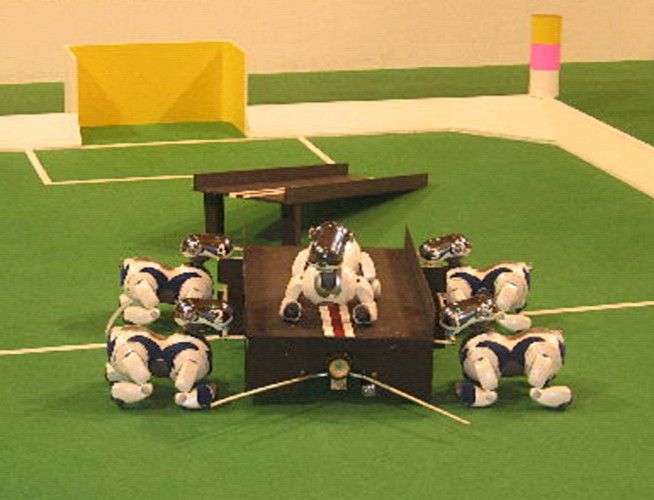
\includegraphics[width=\linewidth]{robocup/robocup.jpg}

% \vspace{-1em}
% \caption{\scriptsize Scene from the SPL Open Challenge~\cite{Dahm2004}.}
% \end{figure}
% }

\vspace{1em}

\begin{center}
\rule{2cm}{0.4pt}\\[0.5em]
\end{center}

\fc{kerdels2013b}{publications/2013-01/2013-01}\nombestpaper\\[1em]
\fc{kerdels2015b}{publications/2015-01/2015-01}\\[1em]
\fc{Kerdels2016}{publications/2016-01/2016-01}\\[1em]
\fc{Kerdels2016a}{publications/2016-03/2016-03}\bestpaper\\[1em]
\fc{Kerdels2016c}{publications/2016-04/2016-04}\nombestpaper\\[1em]
\fc{kerdels2017}{publications/2017-01/2017-01}\\[1em]
\fc{Kerdels2018b}{publications/2018-02/2018-02}\\[1em]
\fcn{Kerdels2018c}{publications/2018-03/2018-03}\\[1em]
\fc{Kerdels2019}{publications/2019-02/2019-02}\\[1em]
\fc{Kerdels2019a}{publications/2019-01/2019-01}

\end{frame}



% The dissertation was featured on the title page of ``Informatik 
% Spektrum''~\cite{Kerdels2018c}, the main organ of the German Informatics 
% Society~(GI).




\begin{frame}{Title \sof{1}{2}}

%\vspace{1em}
\justifying

Foo

\vspace{2em}

% \twocol{0.5}{
% \justifying
% Our technical report~\cite{Dahm2004} provides an in-depth look into the core
% challenges of teaching robots to play soccer, the solutions developed by our
% team, and the involved support infrastructure. 

% \vspace{1em}
% As part of the GermanTeam -- a collaboration between the universities of Berlin,
% Bremen, Darmstadt, and Dortmund -- we won the world championship in the SPL 
% as well as the SPL Open Challenge.

% }{0.41}{
% \vspace{-1.75em}
% \begin{figure}
% 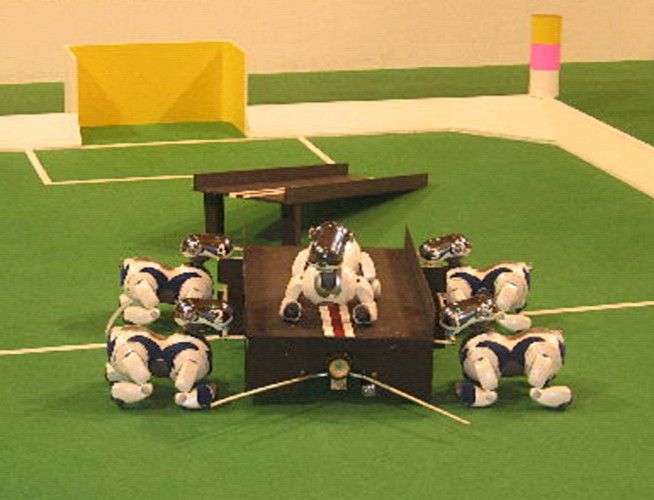
\includegraphics[width=\linewidth]{robocup/robocup.jpg}

% \vspace{-1em}
% \caption{\scriptsize Scene from the SPL Open Challenge~\cite{Dahm2004}.}
% \end{figure}
% }

\vspace{1em}

\begin{center}
\rule{2cm}{0.4pt}\\[0.5em]
\end{center}

\fc{kerdels2013b}{publications/2013-01/2013-01}\nombestpaper\\[1em]
\fc{kerdels2015b}{publications/2015-01/2015-01}\\[1em]
\fc{Kerdels2016}{publications/2016-01/2016-01}\\[1em]
\fc{Kerdels2016a}{publications/2016-03/2016-03}\bestpaper\\[1em]
\fc{Kerdels2016c}{publications/2016-04/2016-04}\nombestpaper\\[1em]
\fc{kerdels2017}{publications/2017-01/2017-01}\\[1em]
\fc{Kerdels2018b}{publications/2018-02/2018-02}\\[1em]
\fcn{Kerdels2018c}{publications/2018-03/2018-03}\\[1em]
\fc{Kerdels2019}{publications/2019-02/2019-02}\\[1em]
\fc{Kerdels2019a}{publications/2019-01/2019-01}

\end{frame}



% The dissertation was featured on the title page of ``Informatik 
% Spektrum''~\cite{Kerdels2018c}, the main organ of the German Informatics 
% Society~(GI).


%%%%%%%%%%%%%%%%%%%%%%%%%%%%%%%%%%%%%%%%%%%%%%%%%%%%%%%%%%%%%%%%%%%%%%%%%%%%%%%%
%%%%%%%%%%%%%%%%%%%%%%%%%%%%%%%%%%%%%%%%%%%%%%%%%%%%%%%%%%%%%%%%%%%%%%%%%%%%%%%%

\begin{frame}[allowframebreaks]{References}

\printbibliography
\end{frame}

\end{document}
